\chapter{Metoder}
Metode kapitlet beskriver projektets arbejdsmetoder, hvilke metoder der brugt og hvordan de er blevet brugt. Metodeafsnittet vil især beskrive projektstyringsforløb og udviklingsmetoderne. 

\section{Projektstyring} \label{title:projektstyring}
Til overordnede projektstyring er der gjort brug af den \textit{Struktureret Agile Metode}, forkortet SAM. (Se hjemmeside \fixme{Reference til http://www.agilemanifesto.org/iso/dk/}). Metoden karakteriseres ved at inddele projektet i følgende faser: krav, design, implementering og test. Metoden passede godt på projektet i flere omstændigheder. SAM er oplagt til projektgrupper i størrelsen 2-3 personer og projekter der varer 3-9 måneder. Metoden er også særlig anvendelig til projektet da inddragelse af kunden fylder en stor del i arbejdet. 
Især i arbejde med forprojektet og opstartsfasen på projektet blev der afholdt mange møder for at fastlægge projektets rammer og kravene til produktet. I SAM metoden adskiller man møder i forskellige kategorier og de tre kategori er som følger: \textit{introduktionsmøde, planlægningsmøde og kontraktmøde}. Samarbejdet med kunde Rolf Blauenfeldt kan meget vel inddeles i tre forskellige møde kategorier. I forprojektet afholdte projektgruppen \textit{introduktionsmøde} med kunden for at forventningsafstemme. Da det var på plads og projektgruppen havde besluttet at kundens problemstilling var en opgave som gruppen kunne løse, blev der afholdt flere \textit{planlægningsmøder} for at finde og udspecificerer de  krav som kunden havde til produktet. Disse møder er afholdt over flere omgange, da der undervej i projekt er opstået situation, som ikke var blevet fastlagte. Men efter der var afholdt tilstrækkeligt \textit{planlægningsmøder} igangsatte projektgruppen første fase af SAM metoden og der blev udarbejdet en kravspecifikation(Se afsnit \ref{title:kravspecifikation}). SAM faserne er iterative processer, derfor blev der undervejs i forløbet  foretaget ændring og justeringer i kravspecifikationen. Kort efterfulgt af kravspecifikation er der udarbejdet en accepttest \ref{title:accepttest}, som blev udfyldt da udviklingen af prototypen er færdigt. Inden arbejdet med prototypen begyndte, blev der udarbejdet et system design \ref{title:systemdesign}, for at fastlægge hvordan systemet skulle struktureres. Da system strukturen var fastlagt begyndt implementeringsfasen og slutter med at gennemføre accepttesten. For uddybende information se afsnit \ref{title:udviklingMetode} omkring udviklingsdokumentationen.

\subsection{Scrum/Pivotaltracker} \label{title:scrum}
Til arbejdsfordeling og planlægning af arbejdsopgaver er projektet udarbejde med hjælp af scrum. Der er ikke brugt scrum i direkte forstand. Men hver uge er blevet set som en sprint, hvor der hver mandag er udarbejdet en sprint backlog som skulle udføres i ugens løb. Emnerne til sprint backlogen er bla. taget fra tidsplanen som kan ses som en overordnet projekt backlog. Sidst på ugen er der afholdt møde, hvor der opsamles på ugens arbejdet og hvilke opgaver i sprint backlogen der er blevet løst. Opgaver, der ikke blev løst, er automatisk blevet videreført til næste uges backlog. Hver mandag når der oprettes et sprint backlog er disse opgaver blevet oprettet i projektstyringsværktøjet \textit{pivotaltracker},( se hjemmeside \fixme{https://www.pivotaltracker.com/}). 

\subsection{Samarbejdsaftale}
For at sikre interne forventninger til projektarbejde i gruppen, har gruppens medlemmer lavet og underskrevet en samarbejdsaftale i begyndelse af projektet. \fixme{reference til samarbejdsaftale}

I forbindelse med samarbejdet med reviewgruppen er der også blevet udarbejdet og underskrevet en samarbejdsaftale, for at sikre ens forventning til reviewmøderne. \fixme{reference til samarbejdsaftale med review gruppen}

\subsection{Samarbejdspartnere} \label{title:samarbejdspartnere}
Dette afsnit beskriver projektgruppens samarbejdspartnere igennem projektet. 

\textbf{Kunden og projektudbyder:} Rolf Ankerlund Blauenfeldt er læge ved neurologisk afsnit på Aarhus Universitet (AUH). Samarbejdet med Rolf har primært bestået i specificering af krav til udvikling af \textit{Konditioneringsapparatet} samt faglig ekspert for remote ischemic conditioning (RIC). Desuden det kunden som godkender accepttesten.

\textbf{Vejleder:} Projektvejleder Peter Johansen, har været som faglig vejleder i gennem hele projekt og igennem vejledermøder Peter bistået med faglig kritik løbende. 

\textbf{Reviewgruppe:} Igennem projektet har projektgruppen samarbejdet med en anden projektgruppen, Anders Esager og Anders Toft. Denne gruppe har fungeret som opponent/review gruppe, og hver gang en deadline var nået, fx accepttest, har grupperne reviewet hinanden opgaver, hvorefter et møde er blevet afholdet og rettelserne er blevet gennemgået.  

\textbf{Firma:} Virksomheden Seagul forhandler blodtryksapparatet og har i projektets opstart fungeret som kontaktperson til en kinesisk udviklingsvirksomheden. Det samarbejdet blevet oprettet for at projektgruppen kunne modtage teknisk sparring i udviklingsfasen. 

\textbf{Advokat:} I forbindelse med tavshedspligt (Se afsnit \ref{title:tavshedspligt}) har projektgruppen samarbejdet med juridisk rådgiver Maibrit Lerche Hendriksen fra Aarhus Universitet. Pga. projektgruppen ønskede samarbejde med en reviewgruppe, kunne samarbejdet ikke begynde før reviewgruppen også blev underlagt tavshedspligt 

\subsubsection{Samarbejde med medikoteknisk afd. AUH}
Til udvikling og kalibrering af \textit{Konditioneringsapparatet} har projektgruppen samarbejde med medikotekniske ingeniører  Sara Rose Newell og Steven Brantlov fra Region Midtjylland. Disse har kun bistå med blodtrykssimulator, samt teknisk forståelse af blodtryksmåling. Samarbejdet har bestået i mail korrespondance, samt to møder på medikoteknisk afsnit på AUH, hvor projektgruppen har testet og kalibreret \textit{Konditioneringsapparatet} på blodtrykssimulatoren. 

\subsubsection{Samarbejde med Troels Johansen}
I forbindelse med udvikling af sikkerhedskontrol til konditioneringsapparatet(Se afsnit \fixme{Reference til projektafgrænsning} omkring projektafgrænsninger) har projektgruppen samarbejdet med Troels Johansen fra lungeafdelingen på AUH. Samarbejdet opstod pga. gruppen manglede ekspertviden omkring pulsoximeteri og afklemning 

\subsection{Ugeplan og logbog}
Som del af projektstyringen, udviklingsprocess samt dagbog er der på ugentlig basis udarbejdet en ugeplan i starten af hver uge og hver uge er afsluttet med en logbog. Ugeplanen indholder de opgaver projektgruppen skal løses i ugens løb og logbogen er en opsamling på ugens arbejde. For uden af fungere som sprint backlog i scrum (Se afsnit \ref{title:scrum}) har logbogen også fungeret som en slags dagbog, hvordan projekts forløb konstant er blevet beskrevet. Logbogen har også været særlig anvendeligt forbindelse med rapport skrivning. 

\subsection{Vejldermøde}
Fra projektets opstart blev der aftalt et vejledermøde i alle ulige uger under projektforløbet. Disse møder er blevet brugt til at sikre at projektarbejdet hele tiden var på rette spor, samt faglig vejledning til projektarbejdet. Desuden er vejledermøderne blevet brugt til at få kritik på færdig dokumenter undervej i forløbet. 

\subsection{Tidsplan}
I forbindelse med forprojektet blev der udarbejdet en tidsplan i gantt chart format. Et gantt chart illutreret start og slut dato for hvert af projektet delelementer. Hver række i tidsplanen udgør et delelement, fx. kravspecifikation og accepttesten og hver kolonne udgør én uge. Tidsplanen er løbende blevet opdateret efterhånden som projekt har nået delelementerne.  \fixme{Insæt sidste opdateret tidsplan}

\subsection{Tavshedspligt} \label{title:tavshedspligt}
Pga. af patentundersøgelse har hele projekt været underlagt tavshedspligt og underskrevet tavshedserklæringer med både universitet og neurologisk afsnit. Tavshedspligten har bla. forsinket nogle processer da alle partner skulle være underforstået med fortroligheden inden et samarbejdet kunne begynde. I andre tilfælde hvor et samarbejde har været kortvarig eller der ikke har været til at underskrive tavshedserklæring, har projektgruppen måtte undlade detaljer ved kommunikation med disse samarbejdspartnere. Dette har i nogle tilfælde betyder at hjælpen fra evt. eksperter har været begrænset af manglende forståelse for projektet. Derfor har den igangværende patentundersøgelse været et begrænsning for projektarbejdet i flere omfang. \fixme{Reference til tavshedserklæring}

\section{Versionsstyring}
For at sikre korrekt og brugervenlig versionsstyring af hele projektets versionsstyring blevet håndteret med git \fixme{Reference til git hjemmeside https://github.com/}. Git er versionsstyring primært udviklet til software. Styringen af versionshistorik fungere ved at man opretter et respository, som ligger på en server, og hver gang man ønsker at arbejde på filer en ens repository, skal man synkroniseret så man har senest version liggende. Foretages en ændring i en fil der køres versionshistorik på, skal denne ændres \textit{committes} til ens repository. Hver gang man tilføjer en ændring, skal man skrive hvilken ændring man har foretaget. Resten af versionsstyring foregår automatik i git, og her gemmes automatisk versionsnummer og dato for ændring. Desuden gør git det også nemt at gå tilbage i versionshistorikken og finde tidligere versionen. 
Selvom prototypen \textit{Konditioneringsapparatet} ikke skal medicinsk godkendes, var det en grund til at vælge et detaljeret versionsstyrings system. Hvis et apparat skal medicinsk godkendelse skal der kunne fremvises en versionshistorik over hele projektet. 
Til grafisk interface findes en række program som gør git og versionsstyring mere brugervenlig, og her har det især været brugbart at kunne se forrige ændringer og tilføjelse. Dette har lette projektarbejdet og mindsket uoverensstemmelser med hvilket dokument er nyeste version. 

Udover git er dropbox blev brugt til at dele projektfiler der ikke har behov for versionsstyring. Dette har fx. været videnskabelige artikler, datablade mm. 

\section{Udviklingsværktøjer}
\textbf{Eclipse:} er blevet brugt til software udvikling af \textit{Konditioneringsapparatet}. For at kunne simplificere kommunikation mellem eclipse og arduino boardet, er der blevet brugt et arduino plugin i eclipse. På den måde kan funktionaliteterne fra Arduino IDE bruges, samtidig med at eclipse funktionaliteter, som \textit{auto complete }, fejlhåndtering og projektstruktur også var tilstedet. 

\textbf{Arduino IDE:} er den oprindelig udviklingsplatform til arduino, men pga at en række manglende funktionalitet er dette kun blevet brugt til simple enhedstest og små scripts. 

\textbf{Matlab:} Til databehandling og visning af signaler fra \textit{Konditioneringsapparatet}. Værktøjet er blevet brugt til at plotte tryk kurver fra tryksensoren, samt oscillationerne målt fra manchetten. Dette har været en stor hjælp for signal forståelse og i forbindelse med kalibrering af blodtryksmåleren. 

\textbf{Fritzing:} er blevet brugt til udarbejdet af fumlebræt tegning og schematics over hardware udvikling. Grundet prototype udviklingen har meget arbejdet foregået på fumlebræt, og at kunne dokumentere og "gemme" en opsætning på fumlebrættet har været stor hjælp til bla. fejlhåndtering. Fritzing er et open source program som er udviklet til dokumentation af prototyper. Da programmet er open source har processen med at finde nye komponenter være simple. 

\textbf{Gimp:} Billede redigering program som er blevet brugt til redigering og udarbejdelse af illustrationen. Især i forbindelse med figurer og illustrationer til latex har gimp været anvendeligt til at skabe vektoriserede billeder. 

\textbf{Maple:} Til filter udregning i forbindelse med design af analoge og digitale filtre er det blevet brugt Maple version 2015. Maple er kommercielt computer algebra system. 

\textbf{Modelio:} Alt udvikling af sysML er foregået i Modelio. Modelio adskiller sig fra andre sysML værktøjer, da det ikke er et tegne program, men et programmeringssprog og IDE. Dette betyder at udviklingen af sysML har været begrænset af sproget, men det betyder også at det har været nemmere at overholde sysML standarden. 

\textbf{TexStudio:} Alt dokumentation er blevet udarbejdet i TexStudio. Dette er valgt for at få totalt kontrol over layoutet i dokumentationen og rapporten. LaTeX og TeXStudio gø også arbejdet med et større projekt mere simpel, da arbejdet med små underdokumenter er meget simplet. 


\section{Udviklingsproces} \label{title:udviklingMetode}
Efter den struktureret agil metodes(SAM) fire faser: krav, design, implementering og test (se afsnit \ref{title:projektstyring}) er udviklingsprocessen foregået i denne rækkefølge. Disse fire faser vil blive beskrevet nedenfor.

	\subsection{Kravspecifikation} \label{title:kravspecifikation}
	Kravspecifikation er et dokument der beskriver de krav som produktet skal kunne. Der skelnes mellem funktionelle og ikke funktionelle krav. De funktionelle krav beskriver de essentielle krav for at produktet kan leve op til kundens behov. Et eksempel på et funktionel krav er at apparatet skal kunne afklemme med tryk på 25 mmHg over det systoliske blodtryk. I kravspecifikation er de funktionelle beskrevet via \textit{fully dressed use cases}. En use case beskriver brugen med produktet i scenarier og ved hjælp af disse scenarier beskrives produktets funktionalitet. En \textit{fully dressed use case} indeholder ud over en beskrivelse scenariet også beskrivelse af hvilke aktører der er involveret i scenariet, samt før og efter betingelse for scenariet. I nogle scenarier kan det også være nødvendigt at beskrive undtagelser for forløbet, hvis disse ikke er for trivielle. Aktørerne der indgår i \textit{fully dressed use cases} er beskrevet med en aktørbeskrivelse i kravspecifikation. Her beskrives aktør rollen, og om han er primær eller sekundær. En primær aktør interagerer aktivt med produktet i use casen og er nødvendig for at scenariet lykkes. En sekunder aktør er passivt involveret med use casen og dette kan for eksempel være en patient der skal modtage behandling med et apparat. For at give læseren et overblik over hvordan aktører og use cases er koblet, indeholder kravspecifikation et overordnet use case diagram, hvor alle scenerier er listet og aktørernes rolle er beskrevet med pile forbundet med use cases. 
	De ikke funktionelle krav, er som navnet antyder, krav der ikke er nødvendige for produktets funktionalitet, men de er essentielle for brugervenligheden, sikkerheden og muligheden for at vedligeholde produktet. De ikke funktionelle krav er også hvor produktet bliver mere specifikt. Et eksempel er at produktet skal kunne gemme information omkring konditioneringsforløbet på et SD kort, dette er et funktionel krav. Et ikke-funktionelt krav der sikre brugervenligheden specificerer hvordan den information skal være struktureret i filen på SD kortet. Dette sikre at brugeren får samme datastruktur ved brug af produktet. 
	For at fastlægge rammerne for udseende af prototypen er indeholder kravspecifikationen også illustrationer af bruger interfacet. 
	
	\subsection{Accepttest} \label{title:accepttest}
	Accepttest er en metode og en del af udviklingsprocessen som skabes for at produktet kan leve op til kravspecifikation. Accepttesten er essentielt for produktudviklingen, for den udføres og godkendes i samarbejdet med kunden. Derfor er projektgruppens garanti for at produktet lever op til de aftalt krav. 
	Dokumentet struktureret således at der er en tabel for hver use case, denne tabel indeholder trinnene fra scenariet og hver trin er indeholder en beskrivelse, en test metode, et forventet resultat og til sidste et felt hvor testen kan godkendes. Det samme struktur gælder for de ikke funktionelle krav. 
	
	\subsection{System design} \label{title:systemdesign}
	Dette trin i udviklingsprocessen vedrører designet at \textit{Konditioneringsapparatet}. For at sikre overensstemmelse inden udviklingsprocessen blev igangsat, blev systemets design og arkitektur beskrevet. System designet indeholder først en beskrivelse af alle systemets underdele. Her beskrivelse hvilke dele der skal indgå i systemet for at det lever op til designet.
	For at sikre at alle område i systemet designet blev belyst er der her gjort brug af metoden \textit{4 plus 1 modellen}. Modellen er oprindelig kun beregnet til software men bruges på systemet som helhed. Modellen ser produktet fra fire forskellige synsvinkler og sikre at alle partners interesser er belyst. Det fire synsvinker er som følger: 
	\\ \textit{Logical view}: Denne synsvinkel beskriver systemets funktionalitet via centrale elementer, mekanismer og stadier. \\
	\textit{Process view}: Beskæftiger sig med den ikke funktionelle del af systemet, og hvordan de centrale elementer fra logical view interagerer med hinanden. \\
	\textit{Implementation view}: Denne vinkel involverer udviklerens perspektiv og beskæftiger sig med hvordan software implementeres. \\
	\textit{Deployment view:} Beskriver systemet fra en fysisk synsvinkel, blandt andet hvordan eksekveringen af softwares skal foregå på apparatet og hvordan systemets fysisk setup skal ser ud. \\
	\textit{NB: Beskrivelse af de fire synsvinkler er udklip fra system design dokumentet.} \fixme{Indsæt reference til system design}
	
	I system design dokumentet er der også gjort stor brug af sysML diagram sproget. Sproget er universel blandt ingeniører og letter forståelsen af systemet. I \textit{Logical view} er det udarbejdet state machine diagrammer, som bruges til at beskrive stadierne som produktet kan befinde sig i, samt hvordan der skiftes mellem disse stadier. I \textit{process view} fokuseres der på hvordan systemet dele interagerer med hinanden og til at beskrive denne kommunikation bruges sekvens diagrammer. Der er udarbejdet et sekvens diagram for hver use case. Sekvensdiagrammer beskriver hvordan scenarieret fra use case udføres i mellem systemets dele, samt hvilken information der videregives mellem underdelene. 
	
	\subsection{Implemetering} \label{title:implementering}
	Implementeringen af produktets funktionalitet er beskrevet i implementeringsdokumentet. Dette dokument bruges til at beskrive hvordan systems enkelt software og hardware dele er implementeret og hvordan disse underdele har opnået deres ønskede funktionalitet. Dokumentet har også til formål at fungere som et opslagsværk, så ønsker læseren forståelse for en specifik software eller hardware del, står det i implementeringsdokumentet. Derfor skal implementeringsdokument også ses som en \textit{opskrift} på hvordan produktet er fremstillet. Dokument indeholder især erfaringen omkring arbejdet med systemets dele og hvordan de væsentlig dele er blevet enhedstestet. 

\subsection{V-model}
Den struktureret agile metode (SAM) indeholder samme faser som V modellen, men beskriver ikke på samme den iterative del af processen. V-modellen beskriver den iterative process (Se figur \ref{fig:vmodel}). Modellen foreskriver at man starter med kravspecifikation og bevæger sig ned mod implementering hvorefter man projektet arbejdet op i mod accepttesten. Pilene i mellem beskriver at arbejdsprocessen er iterativ og fx de nederste 3 kasser; detaljeret design, implementering og unit test er den iterative process meget brugbar. Når opdages en fejl i implementering ændres designet og der gennemføres en ny enhedstest.  
\begin{figure}[H]
	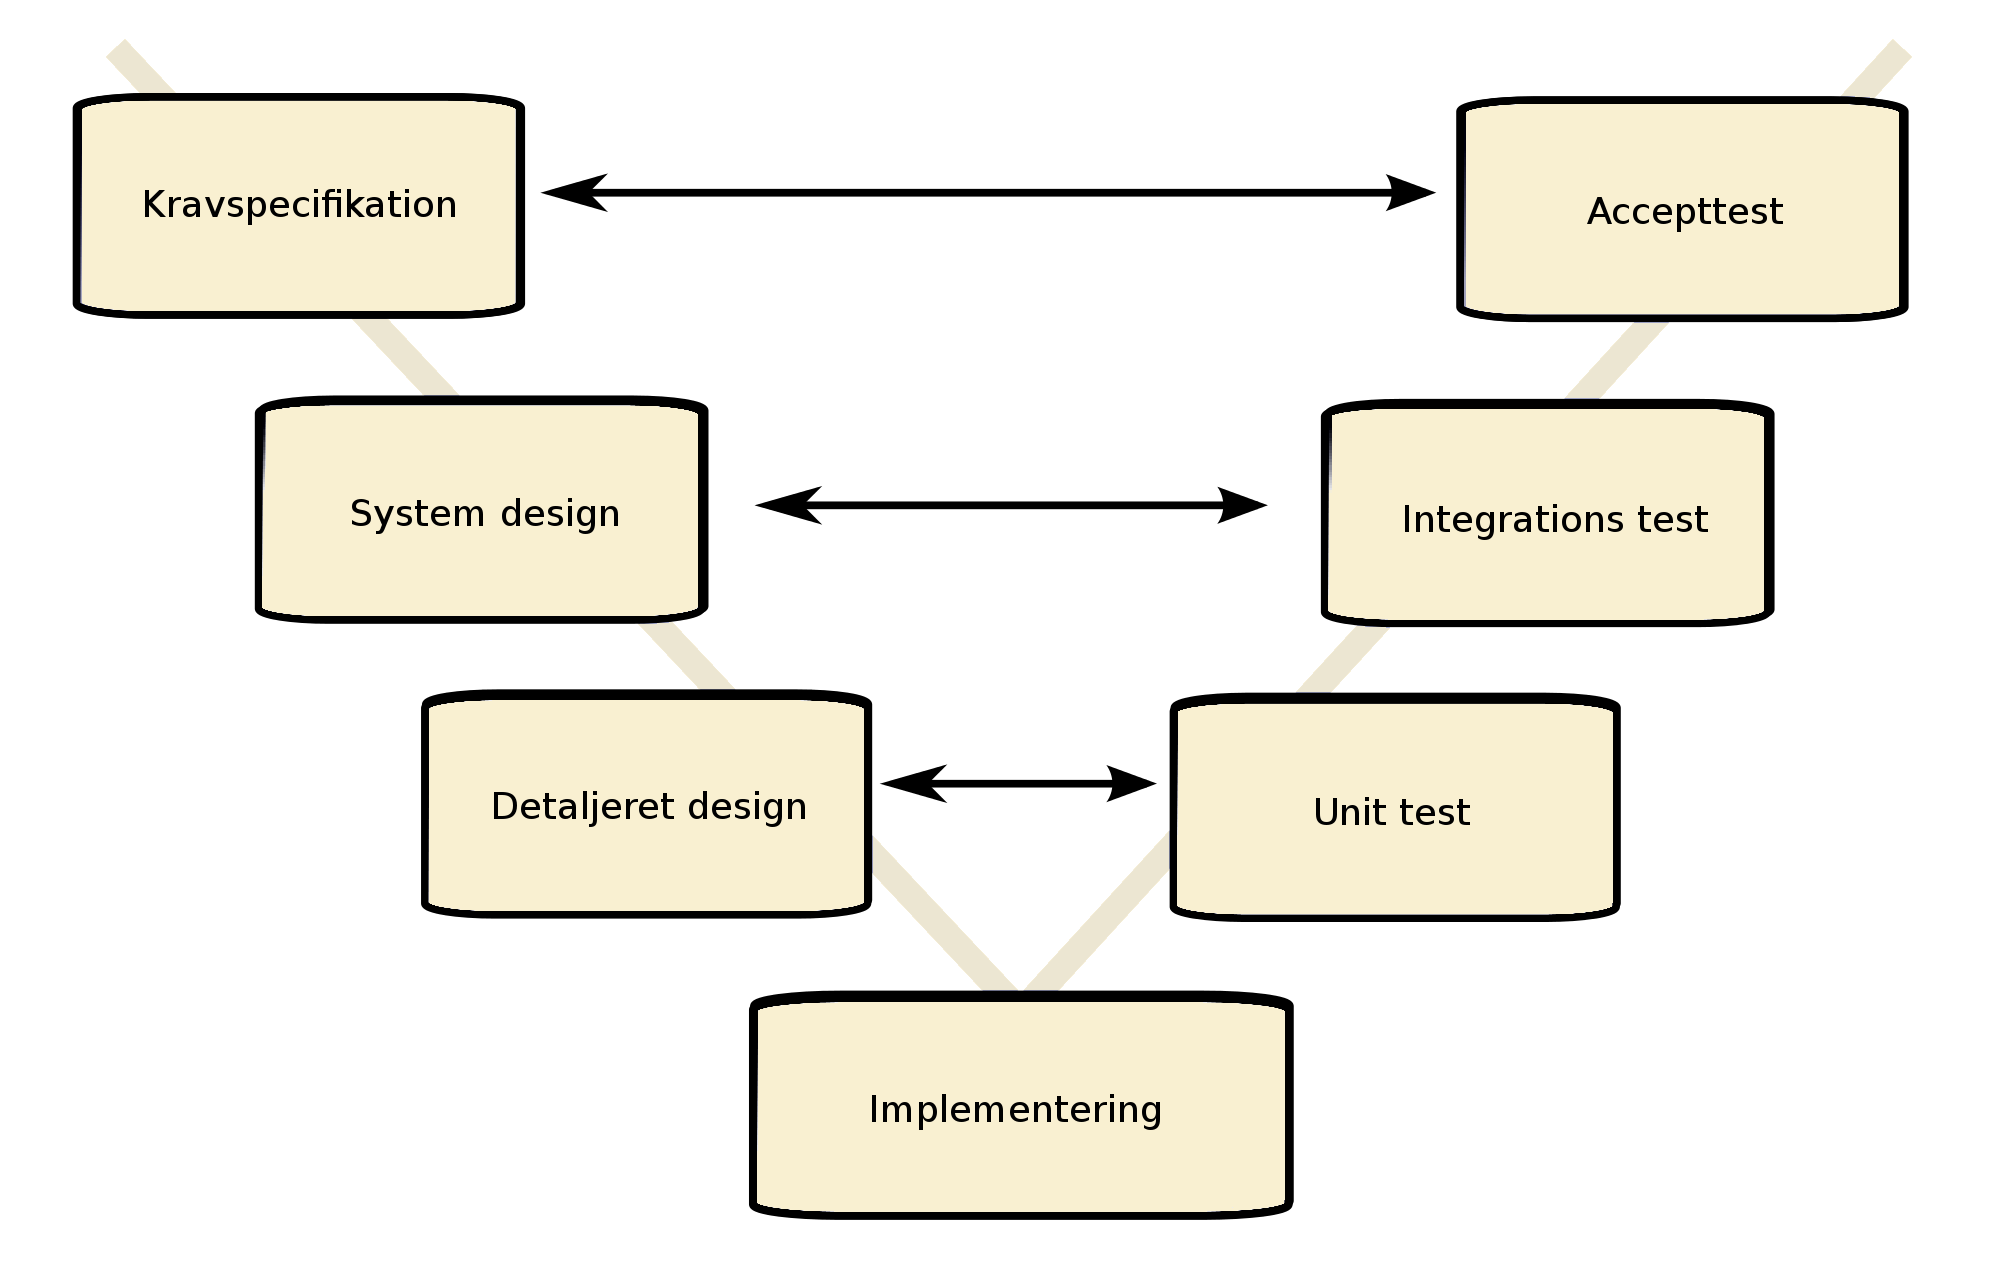
\includegraphics[width = \textwidth]{billeder/vmodel.png}
	\caption{V-modellen}\label{fig:vmodel}
\end{figure}

\subsection{Review}
Review gruppen er beskrevet under afsnittet \ref{title:samarbejdspartnere}. Men review har også været en metode i udviklingsprocessen, i sammenfald med tidsplanen har reviewmøderne fungerede som deadline til hvornår bestemt mål skulle nåes i udviklingsprocessen. 
